\documentclass[aps,rmp,reprint,superscriptaddress,notitlepage,10pt]{revtex4-1}
\usepackage[utf8x]{inputenc}
\usepackage{amsmath,amsthm,amsfonts,amssymb,amscd}
\usepackage{graphicx}
\usepackage{wrapfig}
\usepackage{enumerate}
\usepackage[final]{hyperref}

\newcommand{\avg}[1]{\langle #1 \rangle}
\newcommand{\Lcore}{L_\text{core}}
\newcommand{\Lpang}{L_\text{pang}}
\newcommand{\Lgen}{L_\text{gen}}
\newcommand{\dcore}{\langle d_\text{core} \rangle}

\begin{document}
%\title{PanGraph: scalable multiple genome alignment for pan-genome analysis}
\title{PanGraph: scalable bacterial pan-genome graph construction}
\author{Nicholas Noll}
\affiliation{Kavli Institute for Theoretical Physics, University of California, Santa Barbara \looseness=-5}
\author{Marco Molari}
\affiliation{Swiss Institute of Bioinformatics, Basel, Switzerland \looseness=-5}
\affiliation{Biozentrum, University of Basel, Basel, Switzerland \looseness=-5}
\author{Richard A.~Neher}
\affiliation{Swiss Institute of Bioinformatics, Basel, Switzerland \looseness=-5}
\affiliation{Biozentrum, University of Basel, Basel, Switzerland \looseness=-5}

\begin{abstract}
    The genomic diversity of microbes is commonly parameterized as population genetic polymorphisms relative to a reference genome of a well-characterized, but arbitrary, isolate.
    Reference genomes contain a fraction of the microbial \emph{pangenome}, the set of genes observed within \emph{all} isolates of a given species, and are thus blind to both the dynamics of the accessory genome, as well as variation within gene order and copy number.
    With the wide-spread usage of long-read sequencing, the number of high-quality, complete genome assemblies has increased dramatically.
    Traditional computational approaches towards whole-genome analysis either scale poorly, or treat genomes as dissociated bags of genes, and thus are not suited for this new era.
    Here, we present \emph{PanGraph}, a Julia based library and command line interface for aligning whole genomes into a graph, wherein each genome is represented as an undirected path along vertices, which in turn, encapsulate homologous multiple sequence alignments.
    The resultant data structure succinctly summarizes population-level nucleotide and structural polymorphisms and can be exported into a several common formats for either downstream analysis or immediate visualization.
\end{abstract}

\maketitle

% TODO: check consistency of numberings of figures and sections between SI and main text
% TODO: real data
% TODO: - dataset
% TODO:     - table
% TODO: - size
% TODO:     - figure
% TODO: - benchmark
% TODO:     - figure
% TODO: - marginalization
% TODO: 
% TODO: Table: leave all the columns? Improve description? Depending on what is useful afterwards
% TODO: SI Section IIA: superfluous?
% TODO: minimap2 asm10 superfluous?

%\section{Introduction}
During evolution, microbial genomes change by both local modifications and large-scale alterations \cite{arnold2021horizontal}.
Local mutations conserve sequence architecture and only change a few nucleotides by substitution, insertion or deletion.
Conversely, large-scale mutations reorganize the sequence, and involve either the homologous recombination of large segments or wholesale gene loss or gain from the environment.
The accumulation of such polymorphisms over time complicates comparative genomic analyses of present day isolates; microbial genomes are mosaics of homologous sequence, locally related by an asexual phylogenetic tree \cite{sakoparnig2021whole}.
%Scalable inference techniques of this complicated relatedness structure would, in part, spur the advance of critical epidemiological surveillance tools, analogous to NextStrain, for bacterial pathogens.

Recent advances in long-read sequencing have enabled the low-cost assembly of isolated genomes at the quality of reference databases \cite{whibley2021changing}.
The accumulation of many complete genomes promises to rapidly improve our ability to quantify the evolutionary dynamics that drive microbial diversity in natural populations.
Unfortunately, comparative genomic analyses have not kept pace with the technological advance, opting either for reference-based approaches that only partially capture microbial diversity \cite{tettelin2008comparative}  or to construct a \emph{pangenome} that accurately captures nucleotide polymorphisms within genes but approximates structural polymorphisms as simple gene presence-absence relationships \cite{page2015roary,ding2018panx} .
This new era of pangenomics demands novel data structures to encapsulate the \emph{complete} diversity of a given genomic sample set.

In recent years, efforts have focused on generalizing the \emph{pangenome} framework of microbial diversity to graphical models \cite{eizenga2020pangenome}.
At a high level, pangenome graphs generalize the reference sequence coordinate system conventionally used; microbial diversity is, instead, encapsulated by a graph-based data structure, with vertices or edges labelled by homologous DNA sequences, in which a walk recapitulates a subset of mosaic genomes.
As such, pangenome graphs can be thought of as an analogous construct to the well-known assembly graph, in which whole genomes are individual ``reads" of the underlying microbial structure \cite{myers2005fragment}.

While easy to conceptualize, the construction of pangenome graphs has proven computationally challenging.
Colored generalizations of the de Bruijin graph-based assemblers have been successively used to build graphs from large sequence sets, however the underlying efficiency derives from a fixed kmer size which prevents modelling long-range homology \cite{iqbal2012novo,muggli2017succinct}.
An orthogonal approach has been to formulate the inference of the pangenome graph as a multiple genome alignment.
However, current methods either scale poorly to large sets of genomes \cite{darling2010progressivemauve}, focus on comparisons across diverse sets of species across the tree of life at the cost of memory \cite{armstrong2020progressive}, or utilize a reference-guided approach by partitioning genomes first into annotated genes \cite{gautreau2020ppanggolin,colquhoun2021pandora}.

Here we present PanGraph, a Julia \cite{bezanson2017julia} library and command line interface, designed to efficiently align large sets of closely related genomes into a pangenome graph on personal computers.
The resulting graph both compresses the input sequence set and succinctly captures the population diversity at multiple scales ranging from nucleotide mutations and indels to structural polymorphisms driven by inversions, rearrangements, and gene gain/loss.
The underlying graph data structure can be exported into numerous formats for downstream analysis and visualization in software such as Bandage \cite{wick2015bandage}.
%The algorithm, along with extensive documentation, examples, and instructions for installation, are open source and can be found on GitHub.
%We anticipate PanGraph to be immediately useful in understanding microbial evolution in natural populations.

\section{Algorithms and implementation}
\emph{PanGraph} transforms an arbitrary set of genomes into a \emph{graph} that simultaneously compresses the collection of sequences and exhaustively summarizes both the structural and nucleotide-level polymorphisms.
The graph is composed of \emph{pancontigs}, which represent linear multiple-sequence alignments of homologous sequence found within one or more input genomes.
\emph{Pancontigs} are connected by an edge if they are syntenic on at least one input sequence; individual sequences are then recapitulated by contiguous \emph{paths} through the graph.

\emph{PanGraph's} overarching strategy is to approximate multiple-genome alignment by iterative pairwise alignment, in the spirit of progressive alignment tools \cite{darling2010progressivemauve,armstrong2020progressive}.
A guide tree is utilized to linearize the problem's complexity by approximating multiple-sequence alignment as a quenched order of successive pairwise alignments \cite{feng1987progressive}.
Pairwise graph alignment is performed by an all-to-all alignment of the \emph{pancontigs} between both graphs.

\subsection{Guide tree construction}
The alignment guide tree is constructed subject to three design constraints: (i) sequences are aligned sequentially based upon similarity, (ii) the similarity computation scales sub-quadratically with the number of input sequences, and (iii) the resultant tree is balanced.
To this end, we formulate the algorithm as a two step process.
The initial guide tree is constructed by neighbor-joining \cite{saitou1987neighbor}; the pairwise distance between sequences is approximated by the Jaccard distance between sequence minimizers \cite{roberts2004reducing}.
Computationally, each sequence can be sketched into its set of minimizers in linear time while the cardinality of all pairwise intersections can be computed by sorting the list of all minimizers to efficiently count overlaps.
Hence, the pairwise distance matrix is estimated in log-linear time.
The final guide tree is constructed as the balanced binary tree constrained to reproduce the topological ordering of leaves found initially.
See Fig \ref{fig:visualization}A for a graphical depiction of the guide tree.

\subsection{Iterative graph alignment}
The iterative pangraph construction is illustrated in Fig.~\ref{fig:visualization}.
The pangraph is initialized as one subgraph per input genome, each representing its respective genome as a single \emph{pancontig}.
Pairs of subgraphs are aligned in a postorder traversal of the constructed guide tree.
The identified homologous intervals of the pancontig are then merged, thereby creating shorter contigs that represent homologous sections of multiple input genomes, see Fig. \ref{fig:visualization}B for a graphical deption.
These steps of pairwise graph alignment and merging of homologous intervals are repeated until the root of the guide tree is reached.

\paragraph{Pairwise alignment.}
Full genome alignment between two closely related isolates is a well-studied problem with many high-quality tools available \cite{li2018minimap2,marccais2018mummer4}.
We chose to use \emph{minimap2} as the core pairwise genome aligner for its proven speed, sensitivity, and easy-to-use exposed library API \cite{li2018minimap2}.
This alignment kernel is included within a custom Julia wrapper, available at \url{github.com/nnoll/minimap2_jll.jl}.
However, we note that \emph{PanGraph} is written to be modular, and additional alignment kernels can be added with ease.
In particular we decided to include the option to use \emph{mmseqs2} \cite{steinegger2017mmseqs2} as an alternative alignment kernel, because of its sensitivity on highly diverged sequences at the cost of higher computational time.
In general, the kernel interface expects two lists of \emph{pancontigs} to align as input and will output a list of putative overlapping alignments between both input lists.

\paragraph{Merging of homologous sequence.}
\emph{Pancontigs} encapsulate linear multiple-sequence alignments which are modelled internally by a star phylogeny, i.e. are assumed to be well-described by a reference sequence augmented by independent SNPs and indels for each contained isolate.
Importantly, during the all-to-all alignment phase, \emph{pancontigs} are aligned based \emph{solely} upon their consensus sequence.
All putative homologous alignments found by \emph{pancontig} alignment are ranked according to the pseudo-energy
\begin{equation}\label{eq:pseudo-energy}
    E = -\ell + \alpha N_c + \beta N_m
\end{equation}
where $\ell$, $N_c$, and $N_m$ denote the alignment length, number of \emph{pancontigs} created by the merger, and number of polymorphisms per genome in the newly created {pancontig} respectively.
See Fig \ref{fig:visualization}B for a graphical definition for each term.
Additionally, $\alpha$ and $\beta$ are hyperparameters of the algorithm, respectively controlling the tradeoff between fragmentation of the graph and the maximum diversity within each block.
Only alignments with negative pseudo-energy are performed.

\begin{figure}[htb]
    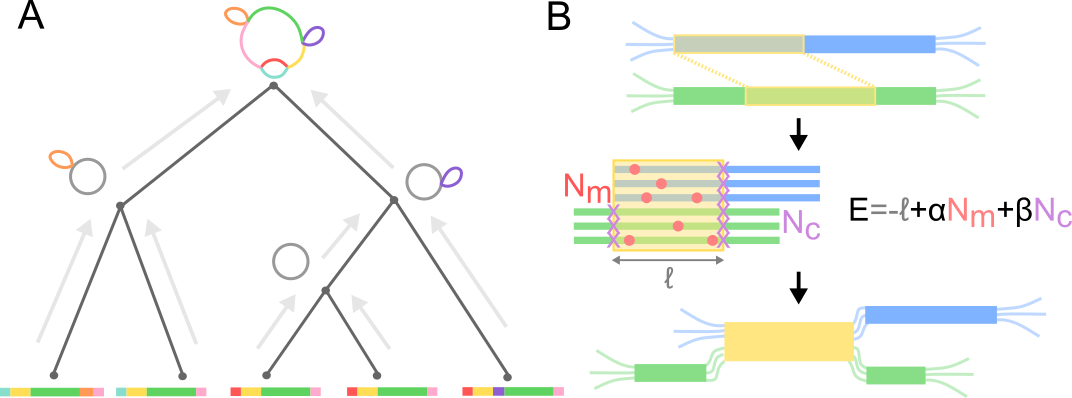
\includegraphics[width=.45\textwidth]{figs/algorithm.png}
    \caption{{\bf Overview of PanGraph algorithm}.
        (A) The alignment graph is constructed progressively by aligning graphs pairwise up a guide tree constructed from neighbor-joining the minimizer overlap between strains.
        (B) During pairwise alignment, \emph{pancontigs} (blue and green)
        are merged by identifying homologous intervals (shown in yellow).
        If the underlying alignments are viewed compatible, i.e. the energy is less than 0, the pancontigs are merged.
    }
    \label{fig:visualization}
\end{figure}

At the graph level, the merger of two \emph{pancontigs} defines a new \emph{pancontig}, connected on both sides by edges to the neighboring \emph{pancontigs} of both inputs, and thus locally collapses the two graphs under consideration.
At the nucleotide level, the pairwise alignment of two \emph{pancontigs} maps the reference of one onto the other; the merger of two \emph{pancontigs} requires the application of the map onto the underlying multiple-sequence alignment.
Once both sets of sequences are placed onto a common coordinate system, the resultant consensus sequence, and thus polymorphisms, are recomputed.
This procedure can be viewed as an online multiple sequence alignment algorithm.

The above procedure is repeated until no alignments with negative energy remain.
Upon completion, transitive edges within the graph are removed by merging adjacent \emph{pancontigs}.

\subsection{Parallelism}
\emph{PanGraph} is designed with a message-passing architecture to enable scalable parallelism, as shown in Fig \ref{fig:visualization}A for a cartoon example.
Each internal node of the guide tree represents a job that performs a single pairwise graph alignment between its two children.
The process will block until both of its children processes have completed and subsequently pass the result of their pairwise graph alignment up to the parent.
All jobs run concurrently from the start of the algorithm; the Julia scheduler resolves the order of dependencies naturally \cite{bezanson2017julia}.
As such, the number of parallel computations is automatically scaled to the number of available threads allocated by the user at the onset of the alignment.

\subsection{Graph Export and Availability}
The constructed pangenome graph can be exported in a variety of file formats for downstream analysis and visualization.
In addition to a custom JSON schema, PanGraph can export the alignment as a GFA file, where each \emph{pancontig} is represented as a segment and each genome as a path.
This allows for visualization in software such as Bandage \cite{wick2015bandage}.
Lastly, we provide functionality to export as a conventional pangenome, however wherein \emph{pancontigs} supplant putative gene clusters, that can be visualized directly by the PanX toolkit \cite{ding2018panx}.
% TODO: add GFA version?

PanGraph is published under an MIT license with source code, extensive documentation, examples, and instructions for installation available at \url{github.com/neherlab/pangraph}.
Additionally, pre-built binaries are available as GitHub releases.
All data and scripts used to validate PanGraph are available within the same repository.
% TODO: add data?

\section{Validation and performance}

\subsection{Validation on synthetic data}

As a first validation step we use generated synthetic data to quantify the performance characteristics of \textit{PanGraph} as a function of input size, and its accuracy as a function of sequence diversity.

\paragraph*{Generation of synthetic data}

We simulated populations of size $N=100$ and sequence length $L=50\,000$ utilizing a Wright-Fisher model \cite{hudson2002generating} evolved for $T=50$ generations.
In addition to nucleotide mutations that occur at rate $\mu$ per generation, we modelled inversions, deletions (respective rates $0.01$ and $0.05$ per generation), and horizontal sequence transfer that occurs with tunable rate $h$ per generation per genome (see SI Section I for details).
The ancestral state for each sequence is tracked through each evolutionary event so that the true mosaic relatedness structure can easily be converted to a graph.
The simulation framework is distributed within the PanGraph command line toolsuite for external use.

\paragraph*{Performances as a function of dataset size}

The algorithmic complexity was measured empirically by simulating populations of increasing size and average sequence length, and generating pangenome graphs for the resulting sequences.
The mean and standard deviation of results obtained from 50 iterations are shown in Fig. \ref{fig:toy-performance}.
Importantly, PanGraph's computational complexity grows \emph{linearly} with the number of input genomes.
We note that the PanGraph scales approximately log-linear with average sequence length, as expected from the underlying algorithmic complexity of \textit{minimap2} \cite{li2018minimap2}.
Benchamrks of CPU and memory usage are reported in SI Section IIA.

\begin{figure}[htb]
    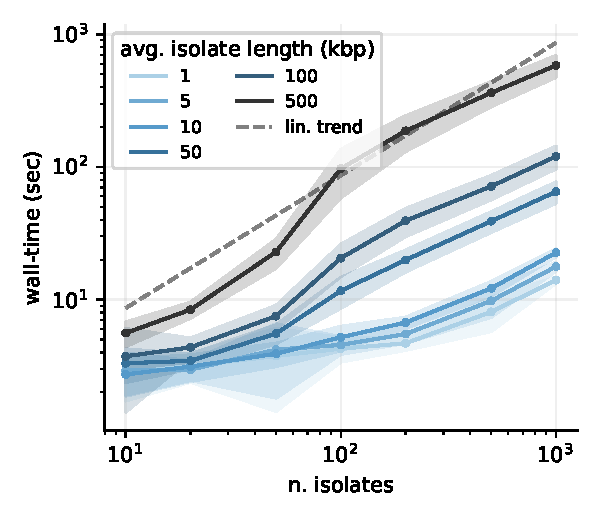
\includegraphics[width=.4\textwidth]{figs/benchmark.pdf}
    \caption{{\bf Algorithm performance}.
        PanGraph scales linearly with the number of input genomes.
        This is a direct result of the guide tree simplification.
        The solid line and ribbons display the mean and standard deviation over 50 runs.
        All runs were performed utilizing 8 cores.
    }
    \label{fig:toy-performance}
\end{figure}

\paragraph*{Accuracy as a function of sequence divergence}

We quantified the accuracy of PanGraph algorithm by computing the displacement of the inferred breakpoints relative to their known locus stored from the evolutionary simulation (cf. SI Section IIB for details). We evaluate this displacement by generating datasets with different rates of mutation $\mu$ and HGT $h$. For each $(h,\mu)$ pair we perform 25 different simulations, and build pangenome graphs using three different options for the alignment kernel, namely \textit{minimap2} \cite{li2018minimap2} with \textit{asm10} and \textit{asm20} option and \textit{mmseqs2} \cite{steinegger2017mmseqs2}.
Critically, we found that the accuracy was \emph{independent} of the rate of horizontal gene transfer $h$ and thus underlying graph complexity. The predominant determinant of accuracy was the sample diversity, controlled by the mutation rate $\mu$ in our simulations (cf. SI Fig.~2). For low-diversity samples breakpoints are inferred with accuracy of few basepairs, while for highly diverged isolates most breakpoints are displaced by several hundreds of basepairs (cf. SI Fig.~3). The choice of alignment kernel influences the threshold diversity at which accuracy is lost.\\
For each alignment kernel and value of average sequence divergence in the population we evaluated the fraction of breakpoints that have displacement greater than the default precision threshold for Pangraph of 100 bp, displayed in Fig.~\ref{fig:toy-accuracy}. On the sequences generated by our simulations, \textit{minimap2} with option \textit{asm20} show a loss of accuracy at a threshold pairwise divergence of around 5\%, while \textit{mmseqs2} is accurate up to average sequence divergence of around 12\%, at the cost of higher computational time.

\begin{figure}[htb]
    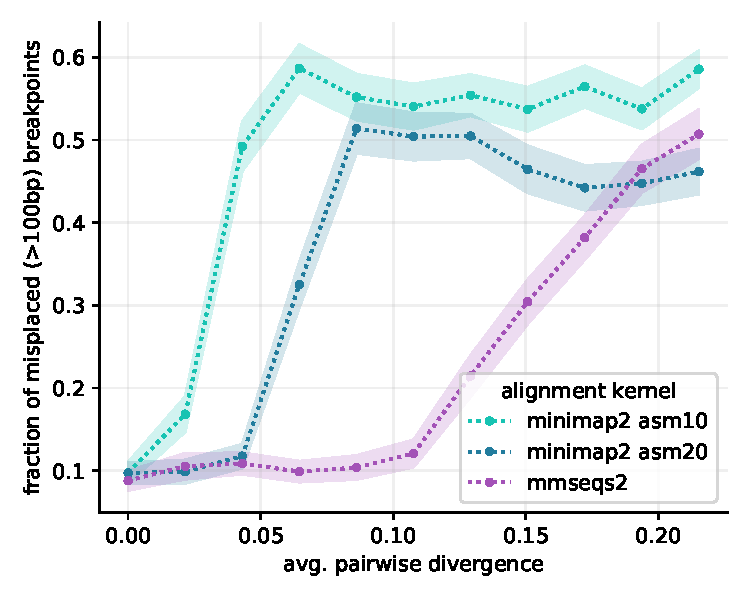
\includegraphics[width=.4\textwidth]{figs/misplaced_fraction_vs_divergence.pdf}
    \caption{{\bf Accuracy against synthetic data}.
        We generate artificial data with varying degree of sequence divergence, and compare the real underlying pangenome graph with the one reconstructed by \textit{PanGraph}, for three different alignment kernels :\textit{minimap2} with \textit{asm10} and \textit{asm20} option, and \textit{mmseqs2}. In each comparison we evaluate the misplacement of breakpoints that we can pair on the two graphs within 1kbp. The plot displays the fraction of breakpoints that have misplacement greater than the standard \textit{PanGraph} precision threshold of 100bp, as a function of average pairwise sequence divergence. Line and shaded area represents mean and standard deviation over 25 repetitions. \textit{mmseqs2} maintains accuracy at higher divergence, at the cost of more computational time.
    }
    \label{fig:toy-accuracy}
\end{figure}


\subsection{Validation on real data}

We additionally validated PanGraph on natural populations sampled from RefSeq \cite{o2016reference}, focusing on the properties of the resulting pangenome graphs for datasets of different size and diversity.

\paragraph*{Dataset characterization}

We downloaded from RefSeq \cite{o2016reference} completely assembled chromosomes from 5 different bacterial species: \textit{Escherichia Coli} (EC), \textit{Klebsiella Pneumoniae} (KP), \textit{Helicobacter Pylori} (HP), \textit{Mycobacterium Tuberculosis} (MT) and \textit{Prochlorococcus Marinus} (PM). These data had been previously analyzed using PanX \cite{ding2018panx}, which allowed us to estimate the size of the pangenome and core genome, and the average pairwise divergence on core genes (cf. Table~\ref{table:panx-dataset} and SI Section~IIIA).
% The \textit{E.~Coli} (EC) dataset is the one with the highest number of isolates (307 chromosomes) and the largest pangenome. The species with the highest core genome divergence are \textit{H.~Pylori} (HP) and \textit{P. Marinus} (PM). For the former, the divergce sits at the limit of what the \textit{minimap2} alignment kernel is able to accurately merge (cf. Fig.~\ref{fig:toy-accuracy}), while for the latter the diversity is beyond even the limits of \textit{mmseqs2}.



\begin{table}[h]
    \setlength{\tabcolsep}{6pt}
    \begin{tabular}{l c c c c c }
        \hline\hline
        Species         & N.  & $\avg{\Lgen}$ & $\Lpang$ & $\Lcore$ & $\dcore$ \\
        \hline
        E.~Coli         & 307 & 5.0           & 17.7     & 0.7      & 1.6\%    \\
        K.~Pneumoniae   & 109 & 5.3           & 13.0     & 2.3      & 0.8\%    \\
        H.~Pylori       & 85  & 1.6           & 1.9      & 0.6      & 4.2\%    \\
        M.~Tuberculosis & 51  & 4.4           & 4.1      & 2.4      & 0.03\%   \\
        P.~Marinus      & 10  & 1.8           & 3.3      & 0.7      & 26.9\%   \\
        \hline
    \end{tabular}
    \caption{{\bf Dataset properties}. Columns represent:
        (1) number of isolates,
        (2) average chromosome lenght in Mbps,
        (3) total pangenome legnth in Mbp,
        (4) total core genome length in Mbp,
        (5) average pairwise divergence of core genes.
    }
    \label{table:panx-dataset}
\end{table}

\paragraph*{Benchmark on real data}

Using \textit{PanGraph}, we build multiple pangenome graphs for each species in the dataset (cf. SI Section~IIIB and IIIC). These differ by the alignment kernel used (\textit{minimap2} with \textit{asm10} or \textit{asm20} option, and \textit{mmseqs2}) or by the value of the pseudo-energy parameters $\alpha,\beta$ from eq.~(\ref{eq:pseudo-energy}). Different alignment kernels are expected to reach different accuracy on datasets with different diversities (cf. Fig.~\ref{fig:toy-accuracy}). Moreover the use of null energy parameters ($\alpha = \beta = 0$) is expected to remove the threshold divergence of 10\% associated with the standard values of parameters ($\alpha=100$, $\beta=10$) at the cost of more fragmented pangenome graphs.\\
\textit{PanGraph} can build pangenome graphs comprising hundreds of isolates in a few hours (5-6h for 307 EC isolates with \textit{minimap2} kernel, cf. Fig~\ref{fig:panx-benchmark}A). Use of \textit{mmseqs2} consistently requires longer computational time, but provides higher accuracy when merging highly diverged sequences. This is the case for the HP dataset, whose core genome divergence sits at the limit of what can be accurately merged with the \textit{minimap2} kernel. In this case the use of \textit{mmseqs2} and null energy parameters increases core pangenome fraction, decreases the total pangenome size and and does not compromise the fragmentation of the graph (cf. Fig~\ref{fig:panx-benchmark}B-C and SI Fig.~4). The divergence of the PM datasets sits instead beyond the capabilities of \textit{Pangraph}. In this case none of the alignment kernel reaches satisfactory sequence compression, and only \textit{mmseqs2} combined with null energy parameters is able to retrieve few core pancontigs.\\
For the other species sequence compression is of the order of few percents, graphs contain thousands to tens of thousands of pancontigs, and 50\% of the pangenome sequence is contained in blocks spanning several kbps.
For these species the use of null energy parameters slightly increases merging and sequence compression, at the cost of slightly more fragmented graphs (cf. SI Section IIIC and SI Fig.~4).
Overall this benchmark showcases the capabilities and limits of \textit{PanGraph}, and demonstrates the value of adapting the pseudo-energy parameter and choice of alignment kernel to the expected diversity of the dataset considered.


% TODO: talk more extensively about the meaning of the results?
\begin{figure*}[htb]
    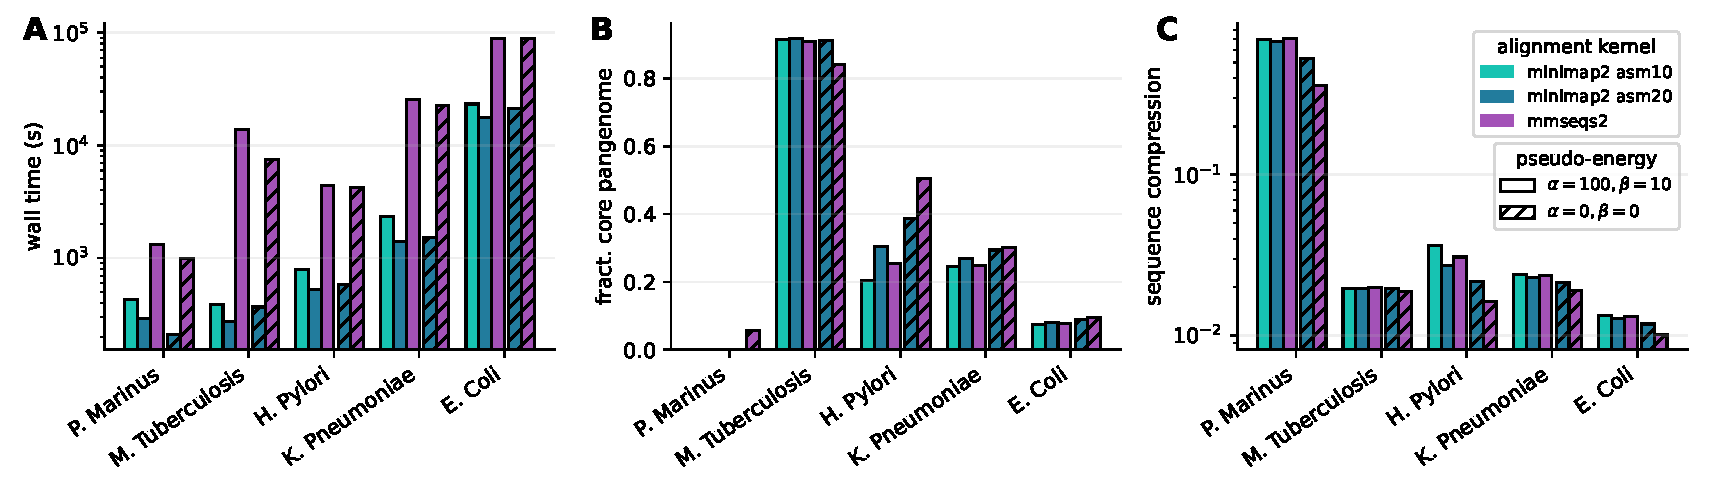
\includegraphics[width=\textwidth]{figs/panx_benchmark.pdf}
    \caption{{\bf Benchmark on real data}.
        We build pangenome graphs from fully-assembled chromosomes from 5 different bacterial species. For each species we build graphs with three different alignment kernel options (\textit{minimap2} with \textit{asm10} or \textit{asm20} option and \textit{mmseqs2}) and two different settings for the pseudo-energy parameters $\alpha, \beta$ (standard or null values).
        \textbf{A}: \textit{PanGraph} wall-time when run in parallel on 8 cores.
        \textbf{B}: fraction of core pangenome in the pangenome graph.
        \textbf{C}: sequence compression, defined as the ratio between the pangenome graph size and the cumulative size of all the sequences contained in the graph.
    }
    \label{fig:panx-benchmark}
\end{figure*}

\paragraph*{Scaling with dataset size}

We then explore how the properties of the pangenome graph scale with the dataset size. To do so we build pangenome graphs from random sets of isolates of increasing size from the EC dataset. Graphs are built with standard values of the parameter and using the \textit{minimap2} kernel with \textit{asm20} option. For each size 10 different random graphs are constructed. Results are reported in Fig.~\ref{fig:panx-size}.\\
The number and size of pancontigs scales sub-linearly with the number of isolates, with most of the pangenome being included in ~10\% of the pancontigs, and core pancontigs having higher-than-average size. Adding more strains does not generate excessive fragmentation of these pancontigs, and their size remains of several kbps even as hundreds of strains are added. The size of the core genome does not decrease significantly with the addition of new strains, while the total pangenome size remains orders of magnitude smaller than the total size of all genomes included in the graph.


\begin{figure*}[htb]
    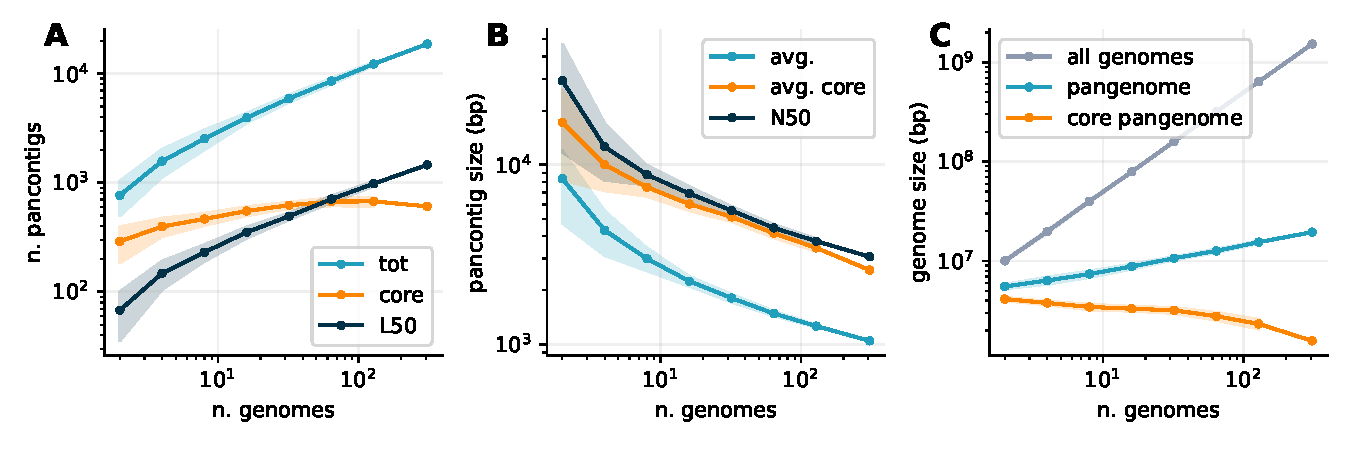
\includegraphics[width=.9\textwidth]{figs/incr_size.pdf}
    \caption{{\bf Pangenome graph properties vs. dataset size}.
        We build pangenome graphs with increasing number of isolates from the E.~Coli dataset and measure the scaling of different properties of the graphs. Lines and shaded areas represent mean and standard deviation over 10 different repetitions on random subsets of isolates, except for the final point indicating the full graph (307 isolates).
        \textbf{A}: n. of pancontigs in the graph. We count the total number of pacontigs (blue), the number of core pancontigs (orange) and the minimum number of pancontigs that contain more than 50\% of the pangenome (L50, black).
        \textbf{B}: average size of pancontigs (blue), of only core pancontings (orange), and size of the smallest panconting in the minimal set that spans 50\% of the pangenome (N50, black).
        \textbf{C}: cumulative size of all genomes in the pangenome graph (gray), total pangenome size (blue) and size of core pangenome (orange).
    }
    \label{fig:panx-size}
\end{figure*}

\section{Graph marginalization}

The interpretation of a pangenome graph containing hundreds of strains can be challenging. To this end it is often informative to inspect simpler sub-graphs comprising only a small subset of isolates. However building multiple such sub-graphs is computationally intensive. To facilitate this task \textit{PanGraph} provides the \verb|marginalize| command, that can be used to marginalize a large pangenome graph on a small subset of strains, removing all the other paths and merging transitive pancontigs. This operation is computationally much cheaper than building a new graph for the subset of strains considered.\\
To verify that marginalized graphs are compatible with newly-built graphs, we built a pangenome graph for 50 randomly selected strains from the \textit{Klebsiella Pneumoniae} dataset. We then picked 50 random pairs of strains from the same set and built two graphs for each pair: the graph obtained by marginalizing the complete graph on the pair, and the graph built directly from the pair (cf. Fig.~\ref{fig:marginalization}A, top).
We compare these two graphs by considering the partition they generate on the genome of the isolates they include. Each genome is partitioned in pancontigs that are either shared on the pair, or private to one isolate (cf. Fig.~\ref{fig:marginalization}A, bottom). We can classify the segments in the intersection of the two partitions in different categories, depending on whether the two partitions agree on whether the segment is shared or private. Moreover segments on which the two partitions agree are further sub-divided depending on whether they are private or shared on both partitions.\\
Compatibility between the two graphs requires segments on which the two partitions disagree to be few and short. Indeed, we verified that over the pairs we picked these segments cover a very small fraction of the genome ($<1\%$), and have average size compatible with the default 100 bp precision threshold of \textit{PanGraph} (cf. Fig.~\ref{fig:marginalization}B-C). This is contrary to agreement segments, that have average size of several kbps. The prevalence of agreement segment cannot be explained only by the fact that most of the genome is shared, since segments that are shared on both graphs cover on average only 85\% of the sequence. We confirmed this results using the fraction of shared k-mers, using an approach inspired by PopPUNK \cite{lees2019fast}. Namely, we approximate the fraction of homologous sequence between any two pairs using the fraction of shared k-mers (in our case we take $k=21$). This fraction is however an underestimate of the fraction of homologous sequence because of mutations. We therefore correct it with the factor $(1-d)^{-k}$, where $d$ is the average pairwise divergence on core genes for the pair considered. The resulting distribution of shared sequence is indeed in very good agreement with the fraction of segments that are shared on both graphs (cf. Fig.~\ref{fig:marginalization}B), suggesting that homologous sequences are correctly merged on the complete, marginalized and pairwise graphs.\\
We performed the same test on species from the other datasets, obtaining similar results on all species whose divergence is compatible with \textit{PanGraph} capabilities (cf. SI Section IV and SI Fig.~5).


\begin{figure*}[htb]
    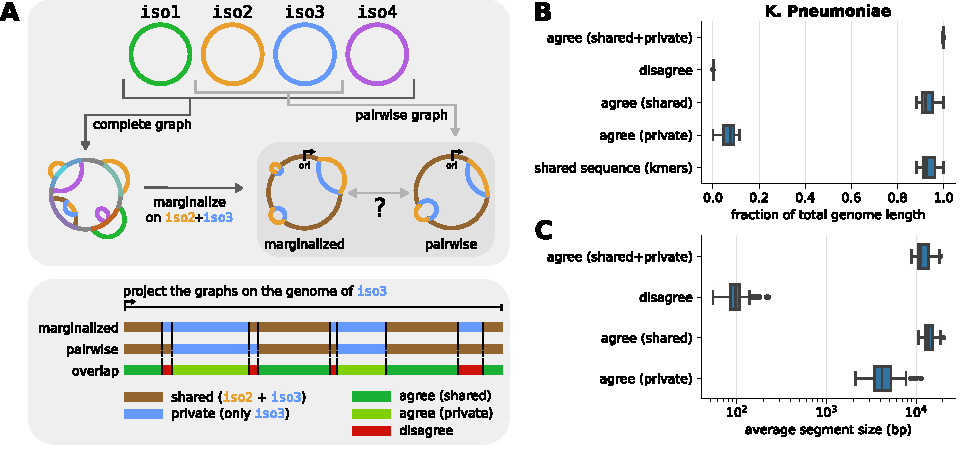
\includegraphics[width=\textwidth]{figs/marginalize_test.pdf}
    \caption{{\bf Test of graph marginalization}.
        \textbf{A}: we built a pangenome graph from 50 randomly chosen strains from the \textit{K. Pneumoniae} dataset. We then randomly picked 50 pairs of strains. For each pair we compared the pangenome graph obtained by marginalizing the complete graph on the pair of strain, and the one obtained by building a new graph for the pair (top). The comparison is done by considering that each graph partitions a genome in shared and private segments. By combining the partitions generated by the marginalized and pairwise graphs we categorize segments in three categories, depending on whether the two partitions agree or not, and if they agree depending on whether segments are shared or private. All graphs were built using \textit{minimap2} alignment kernel with \textit{asm20} option and default value for the energy parameters.
        \textbf{B}: distribution of the average fraction of the genome covered by segments of each category, over the 50 pairs considered (2 entries per pair). The last line represents the distribution of shared sequence, approximated using the fraction of shared k-mers corrected using sequence divergence as described in the main text.
        \textbf{C}: distribution of average segment lengths for each category over the 50 pairs considered (2 entries per pair).
    }
    \label{fig:marginalization}
\end{figure*}



\section{Discussion}

While single nucleotide differences in the core genome are straightforward to analyze with existing tools, these analyses miss the great majority of genetic diversity. The ability to rapidly align large sets of closely related, fully assembled genomes is crucial for the investigation of the processes governing microbial evolution. We developed \textit{PanGraph} as a tool that can extract information on homology, diversity and syntheny, both on core and accessory genome, in a scalable way.

In our analysis we demonstrated the capabilities and limits of this tool, both on synthetic and real sequences. The efficient implementation of \textit{PanGraph} allows it to create pangenome graphs containing hundreds of isolates in a few hours on a 8-cores machine. The size of pancontigs and the fraction of core sequece have good scaling properties with the number of isolates in the graph, indicating that \textit{PanGraph} is able to successfully capture pangenome properties.\\
One of the main limitations is the diversity of the input sequences. The default \textit{minimap2} kernel is able to correctly merge sequences up to around 5\% divergence. Sequences with higher divergence (up to 10-15\%) can be merged using the \textit{mmseqs2} alignment kernel, and tuning the $\alpha, \beta$ energy parameters (cf. eq.~(\ref{eq:pseudo-energy})), trading off speed for sensitivity.\\
We also provide the ability to quickly marginalize big graps on a subset of strains, obtaining simpler graphs that can more easily be explored. Graphs can also be exported in different formats for further analysis and visualization.

We hope that these characteristics will make \textit{PanGraph} a valuable tool, with the potential to spur novel insight on microbial diversity and the processes by which bacteria adapt and change.


\section*{Acknowledgement}
We are grateful to Boris Shraiman for stimulating discussions.
This study was funded by the University of Basel and the NSF.

\bibliography{cite}{}

\end{document}